
\subsection{Fit Procedure}
\label{sec:fit}

A maximum-likelihood fit is performed over the various fit regions described in Section \ref{sec:evt_selection} in order to extract the best-fit value of the WZ + b-jet and WZ + charm jet contributions for events with both 1 and 2 associated jets.

Because the fit regions are defined by the number of associated jets at reco-level, an unfolding procedure is applied to the signal in order to account for differences in the number of truth jets compared to the number of reco-jets. The $WZ$ + b, $WZ$ + charm and $WZ$ + light contributions are separated into independent samples based on the number of truth jets in each event. WZ + 1 truth-jet and WZ + 2 truth-jets are treated as signal samples, while WZ + 0 truth-jets and WZ + $>=$3 truth-jets are treated as an additional background. 

A maximum likelihood fit to data is performed simultaneously in the regions described in Section \ref{sec:evt_selection}, summarized in figure \ref{fig:summary}. The six signal templates, which include WZ+b 1-jet, WZ+c 1-jet, WZ+l 1-jet, WZ+b 2-jets, WZ+c 2-jets, WZ+l 2-jets, are allowed to float, while the remaining background contributions are held fixed. The parameters $\mu_{WZ+b - 1-jet}$, $\mu_{WZ+charm 1-jet}$, $\mu_{WZ+light - 1-jet}$, $\mu_{WZ+b - 2-jet}$, $\mu_{WZ+charm 2-jet}$, $\mu_{WZ+light - 2-jet}$, where $\mu = \sigma_{observed}/\sigma_{SM} $, are extracted from the fit. A simultaneous fit is performed over all 1-jet and 2-jet regions.

\begin{figure}[H]
  \center                                                                                                                    
  \includegraphics[width=.9\linewidth]{sys_truthJets/Plots/Summary_postFit.png}
  \caption{Post-fit summary of the fit regions.}
  \label{fig:summary}
\end{figure}

As described in Section \ref{sec:sys}, there are 230 systematic uncertainties that are considered as NPs in the fit. These NPs are constrained by Gaussian or log-normal probability density functions. The latter are used for normalisation factors to ensure that they are always positive. The expected number of signal and background events are functions of the likelihood. The prior for each NP is added as a penalty term, decreasing the likelihood as it is shifted away from its nominal value. The correlations between these nuisance parameters are summarized in Figure \ref{fig:corr_mat_1j}. 

Several alternative fit strategies are documented in Appendices \ref{sec:incFit}-\ref{sec:inc_tZ}. These include a measurement of WZ + 1 or 2 jets inclusively, a fit where tZ is allowed to float, and a case where tZ is included as part of the signal.

\subsection{Results of the Simultaneous Fit}
\label{sec:resSum}

The Asimov fit for 1-jet events gives an expected $\mu$ value of $1.00^{+0.47}_{-0.43}(stat)^{+0.30}_{-0.27}(sys)$ for $WZ$ + b. The fitted cross-section modifiers for $WZ$ + charm and $WZ$ + light are $1.00 \pm 0.17 \pm 0.17$ and $1.00 \pm 0.06 \pm 0.14 $, respectively.

The expected cross-section of WZ+b with 1-jet is $1.74^{+0.82}_{-0.75}(stat)^{+0.53}_{-0.48}(sys)$ fb, and $14.6 \pm 2.5 (stat) \pm 2.3 (sys)$ fb for WZ + charm, with a correlation of -0.15 between them. An expected significance of 2.0 is observed for WZ + b in this region. 

For 2-jet events, the fit gives an expected $\mu$ value of $1.00^{+0.53}_{-0.51}(stat)^{+0.39}_{-0.34}(sys)$ for $WZ$ + b. The fitted cross-section modifiers for $WZ$ + charm and $WZ$ + light are $1.00 \pm 0.25 \pm 0.21$ and $1.00 \pm 0.06 \pm 0.16 $, respectively.

The expected $WZ$ + b cross-section in the 2-jet region is $2.5^{+1.3}_{-1.3}(stat)^{+0.95}_{-0.83}(sys)$ fb with an expected significance of 1.7$\sigma$. The 2-jet expected cross-section of $WZ$ + charm is $12.7 \pm 3.2 (stat) \pm 2.7 (sys)$ fb, and the correlation between WZ + charm and WZ + b is -0.22. 

A summary of the correlation between the various WZ components is summarized in Table \ref{tab:WZ_corr}.

\hspace{-1in}\begin{table}[H]
\begin{adjustwidth}{-3em}{-3em}
\begin{center}
\begin{tabular}{l|cccccc}
\hline
 & WZ + b - 1-jet & WZ + c - 1-jet & WZ + l - 1-jet & WZ + b - 2-jet & WZ + c - 2-jet & WZ + l - 2-jet\\
WZ + b - 1-jet & 1.00 & -0.15 & 0.28 & -0.13 & -0.22 & 0.17 \\
WZ + c - 1-jet & - & 1.00 & 0.36 & 0.13 & -0.14 & -0.16 \\
WZ + l - 1-jet & - & - & 1.00 & 0.10 & -0.20 & -0.39 \\
WZ + b - 2-jet & - & - & - & 1.00 & -0.22 & 0.17 \\
WZ + c - 2-jet & - & - & - & - & 1.00 & 0.23 \\
WZ + l - 2-jet & - & - & - & - & - & 1.00 \\
\hline
\end{tabular}
\caption{Correlations between the various components of WZ}
\label{tab:WZ_corr}
\end{center}
\end{adjustwidth}
\end{table}

The correlations between the all of the nuisance parameters considered in the fit are summarized in Figure \ref{fig:corr_mat_1j}.a

\begin{figure}[H]                                                                                                            
    \centering                                                                                                               
    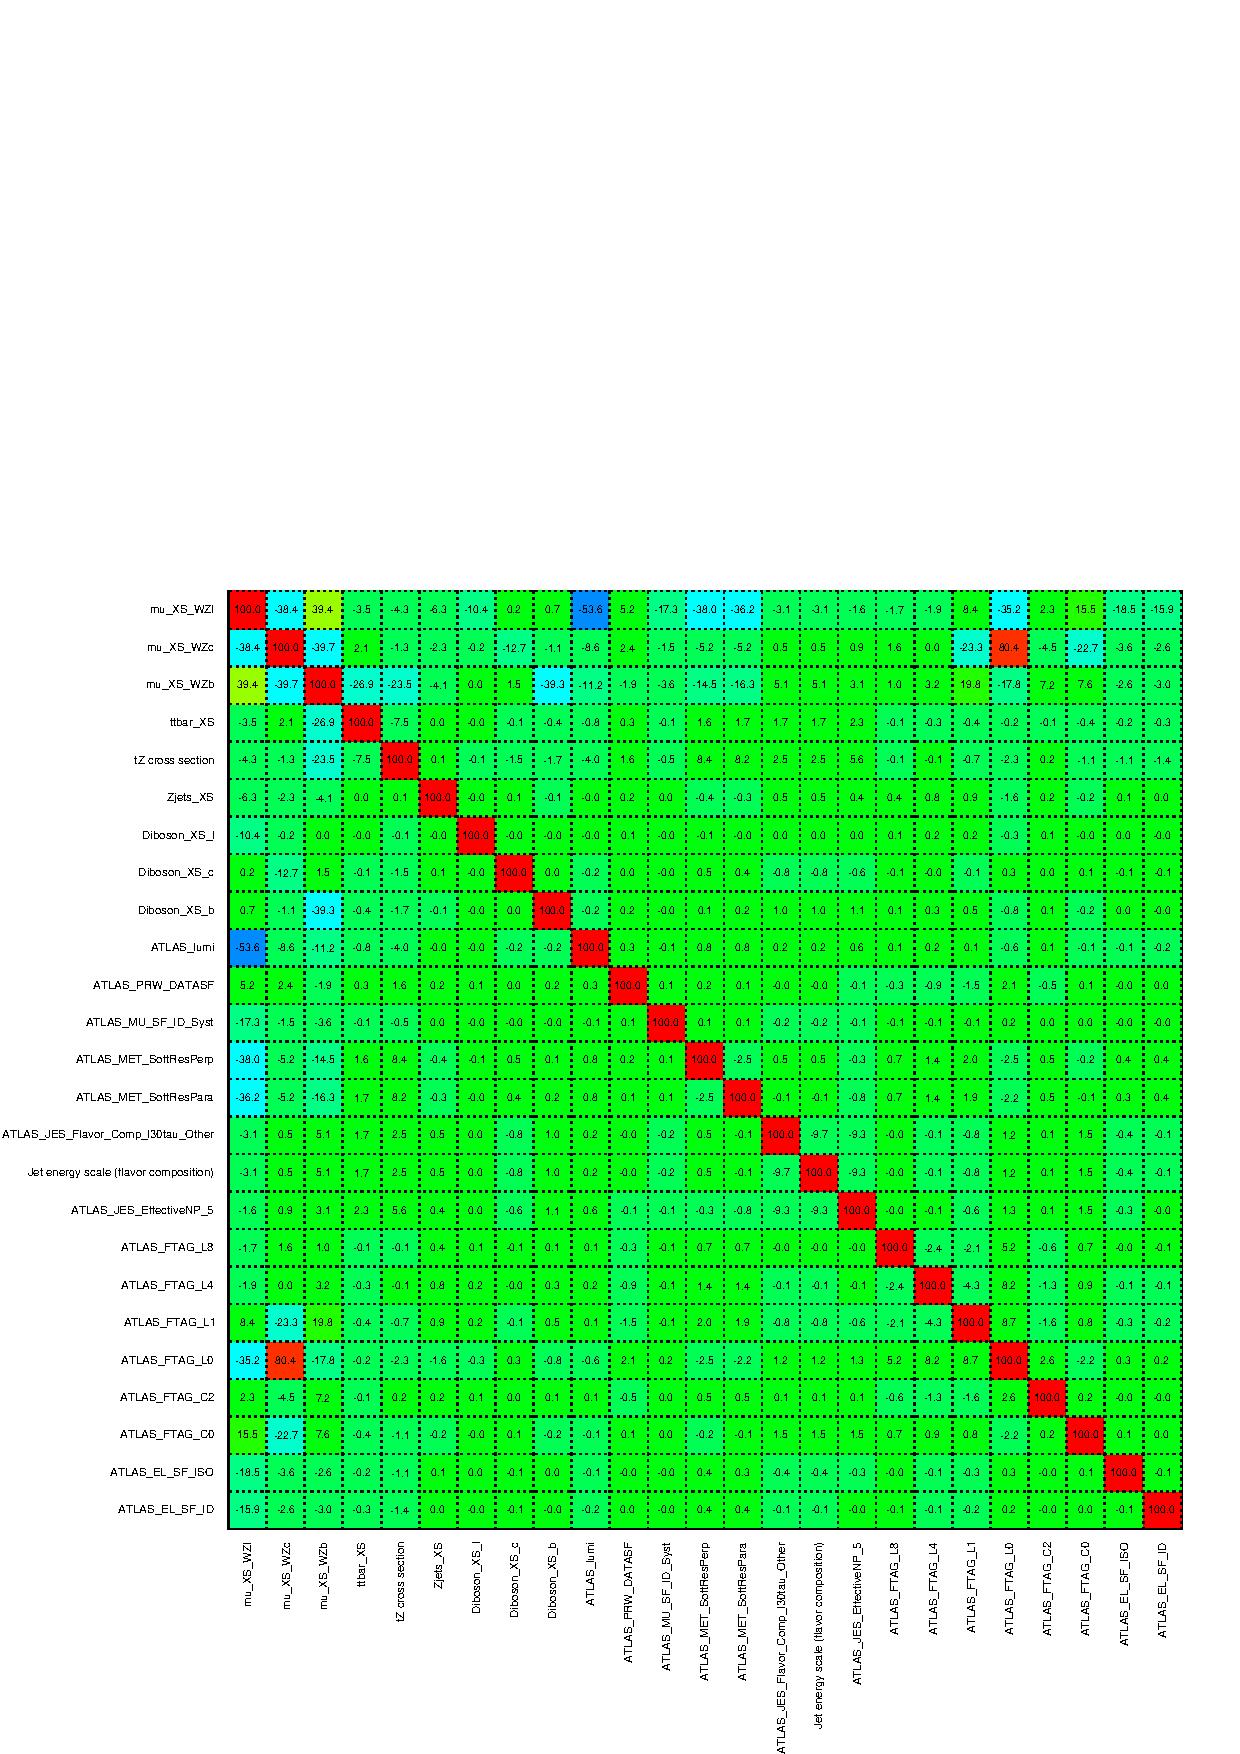
\includegraphics[width=1.0\linewidth]{sys_truthJets/CorrMatrix.png}
    \caption{Correlations between nuisance parameters}
    \label{fig:corr_mat_1j}
\end{figure}


The pre-fit yields in each of the 1-jet regions used in the fit are shown in Table \ref{tab:prefitYield1j}.

\hspace{-1in}\begin{table}[H]
\begin{adjustwidth}{-3em}{-3em}
\small
\begin{tabular}{|l|c|c|c|c|c|c|}
\hline 
Sample & {1j, $<$85\% WP} & {1j, 77\%-85\% WP} & {1j, 70\%-77\% WP} & {1j, 60\%-70\% WP} & {1j, 60\%+ WP} & {tZ CR}\\
\hline 
  $WZ + b - 1j$   & 8.1 $\pm$ 1.6 & 4.7 $\pm$ 0.5 & 4.6 $\pm$ 0.4 & 5.1 $\pm$ 0.4 & 18.1 $\pm$ 2.4 & 5.0 $\pm$ 0.6 \\ 
  $WZ + c - 1j$   & 260 $\pm$ 22 & 81 $\pm$ 6 & 43.1 $\pm$ 3.6 & 25.8 $\pm$ 2.6 & 9.4 $\pm$ 1.8 & 2.9 $\pm$ 0.6 \\ 
  $WZ + l - 1j$   & 3090 $\pm$ 250 & 91 $\pm$ 13 & 17 $\pm$ 3 & 4.9 $\pm$ 1.6 & 1.3 $\pm$ 0.4 & 0.2 $\pm$ 0.1 \\ 
  $WZ + b - 2j$   & 1.10 $\pm$ 0.37 & 0.44 $\pm$ 0.11 & 0.39 $\pm$ 0.06 & 0.62 $\pm$ 0.14 & 2.1 $\pm$ 0.5 & 0.59 $\pm$ 0.14 \\
  $WZ + c - 2j$   & 21 $\pm$ 5 & 5.6 $\pm$ 1.2 & 3.0 $\pm$ 0.7 & 2.0 $\pm$ 0.5 & 0.70 $\pm$ 0.20 & 0.30 $\pm$ 0.08\\
  $WZ + l - 2j$   & 250 $\pm$ 60 & 5.7 $\pm$ 1.6 & 0.73 $\pm$ 0.53 & 0.31 $\pm$ 0.15 & 0.07 $\pm$ 0.06 & 0.01 $\pm$ 0.01 \\
  $WZ - Other$   & 13 $\pm$ 5 & 1.4 $\pm$ 0.4 & 0.42 $\pm$ 0.08 & 0.2 $\pm$ 0.01 & 0.30 $\pm$ 0.05 & 0.67 $\pm$ 0.15 \\
  Other VV   & 6.2 $\pm$ 0.6 & 0.2 $\pm$ 0.4 & 0.2 $\pm$ 0.04 & 0.07 $\pm$ 0.1 & 0.1 $\pm$ 0.1 & 0.1 $\pm$ 0.2 \\ 
  ZZ   & 336 $\pm$ 26 & 17.8 $\pm$ 2.1 & 4.3 $\pm$ 0.6 & 1.7 $\pm$ 0.5 & 0.36 $\pm$ 0.08 & 0.10 $\pm$ 0.03 \\ 
  $t\bar{t}W$   & 1.1 $\pm$ 0.2 & 0.2 $\pm$ 0.1 & 0.3 $\pm$ 0.1 & 0.4 $\pm$ 0.1 & 1.5 $\pm$ 0.3 & 0.7 $\pm$ 0.2 \\ 
  $t\bar{t}Z$   & 6.8 $\pm$ 1.2 & 1.4 $\pm$ 0.3 & 1.0 $\pm$ 0.2 & 1.2 $\pm$ 0.2 & 4.4 $\pm$ 0.8 & 3.2 $\pm$ 0.6 \\ 
  $Z+\text{jets}$   & 169 $\pm$ 38 & 8.9 $\pm$ 1.9 & 3.7 $\pm$ 0.8 & 3.3 $\pm$ 0.7 & 3.2 $\pm$ 0.7 & 0.8 $\pm$ 0.17 \\ 
  $V+\gamma$   & 45 $\pm$ 28 & 1.9 $\pm$ 2.4 & 0.1 $\pm$ 0.1 & 0.02 $\pm$ 0.01 & 1.0 $\pm$ 0.9 & 0.02 $\pm$ 0.03 \\ 
  $tZ$   & 31.8 $\pm$ 4.3 & 6.4 $\pm$ 1.1 & 5.3 $\pm$ 0.8 & 7.2 $\pm$ 1.1 & 11.8 $\pm$ 2.0 & 33.9 $\pm$ 4.5 \\ 
  $tW$   & 1.4 $\pm$ 0.8 & 0.2 $\pm$ 0.5 & 0.0 $\pm$ 0.2 & 0.7 $\pm$ 0.6 & 0.26 $\pm$ 0.42 & 0.39 $\pm$ 0.41 \\ 
  $WtZ$   & 2.3 $\pm$ 1.2 & 0.6 $\pm$ 0.3 & 0.3 $\pm$ 0.21 & 0.27 $\pm$ 0.2 & 1.1 $\pm$ 0.7 & 0.6 $\pm$ 0.5 \\ 
  $VVV$   & 12.4 $\pm$ 0.5 & 0.93 $\pm$ 0.06 & 0.35 $\pm$ 0.03 & 0.13 $\pm$ 0.02 & 0.14 $\pm$ 0.03 & 0.02 $\pm$ 0.01 \\ 
  $VH$   & 40 $\pm$ 6 & 2.6 $\pm$ 1.4 & 0.9 $\pm$ 0.8 & 0.7 $\pm$ 0.8 & 0.5 $\pm$ 0.6 & 0.0 $\pm$ 0.0 \\ 
  $t\bar{t}$   & 12.1 $\pm$ 1.6 & 2.9 $\pm$ 0.6 & 2.5 $\pm$ 0.5 & 2.8 $\pm$ 0.5 & 11.2 $\pm$ 1.4 & 10.9 $\pm$ 1.5 \\ 
  $t\bar{t}H$   & 0.24 $\pm$ 0.03 & 0.05 $\pm$ 0.01 & 0.04 $\pm$ 0.01 & 0.06 $\pm$ 0.01 & 0.20 $\pm$ 0.03 & 0.13 $\pm$ 0.02 \\ 
\hline 
  Total  & 5010 $\pm$ 260 & 227 $\pm$ 24 & 88 $\pm$ 12 & 57 $\pm$ 8 & 76 $\pm$ 16 & 53 $\pm$ 8 \\ 
\hline 
\end{tabular} 


\label{tab:prefitYield1j}
\caption{Pre-fit yields in each of the 1-jet regions.}
\end{adjustwidth}
\end{table}

The post-fit yields in each region are summarized in Figure \ref{tab:postfitYield1j}.

\hspace{-1in}\begin{table}[H]
\begin{adjustwidth}{-3em}{-3em}
\small
\begin{tabular}{|l|c|c|c|c|c|c|}
\hline 
 & {1j, $<$85\% WP} & {1j, 77\%-85\% WP} & {1j, 70\%-77\% WP} & {1j, 60\%-70\% WP} & {1j, $>$60\% WP} & {tZ CR}\\
\hline 
  $WZ + b$   & 11.15 $\pm$ 4.94 & 4.68 $\pm$ 2.00 & 4.61 $\pm$ 1.99 & 5.14 $\pm$ 2.14 & 24.28 $\pm$ 10.11 & 6.01 $\pm$ 2.50 \\ 
  $WZ + c$   & 318.25 $\pm$ 61.13 & 80.74 $\pm$ 14.38 & 43.26 $\pm$ 7.65 & 25.82 $\pm$ 4.87 & 9.40 $\pm$ 2.31 & 2.86 $\pm$ 0.72 \\ 
  $WZ + l$   & 4017.60 $\pm$ 131.71 & 90.52 $\pm$ 11.37 & 17.30 $\pm$ 2.81 & 4.94 $\pm$ 1.58 & 1.25 $\pm$ 0.42 & 0.23 $\pm$ 0.13 \\ 
  Other VV + b   & 0.09 $\pm$ 0.09 & 0.01 $\pm$ 0.22 & 0.01 $\pm$ 0.01 & 0.07 $\pm$ 0.06 & 0.04 $\pm$ 0.10 & 0.03 $\pm$ 0.04 \\ 
  Other VV + c   & 0.67 $\pm$ 0.38 & 0.08 $\pm$ 0.12 & 0.03 $\pm$ 0.03 & 0.07 $\pm$ 0.06 & 0.04 $\pm$ 0.05 & 0.01 $\pm$ 0.01 \\ 
  Other VV + l   & 6.20 $\pm$ 0.64 & 0.19 $\pm$ 0.07 & 0.02 $\pm$ 0.01 & 0.01 $\pm$ 0.01 & 0.01 $\pm$ 0.01 & 0.01 $\pm$ 0.01 \\ 
  ZZ + b   & 1.33 $\pm$ 0.72 & 0.69 $\pm$ 0.39 & 0.49 $\pm$ 0.27 & 1.14 $\pm$ 0.62 & 3.59 $\pm$ 1.89 & 1.04 $\pm$ 0.57 \\ 
  ZZ + c   & 10.27 $\pm$ 5.33 & 2.40 $\pm$ 1.27 & 1.45 $\pm$ 0.80 & 1.01 $\pm$ 0.54 & 0.56 $\pm$ 0.33 & 0.12 $\pm$ 0.09 \\ 
  ZZ + l  & 336.48 $\pm$ 55.34 & 17.81 $\pm$ 3.07 & 4.33 $\pm$ 0.79 & 1.66 $\pm$ 0.35 & 0.36 $\pm$ 0.12 & 0.10 $\pm$ 0.05 \\ 
  $t\bar{t}W$   & 1.09 $\pm$ 0.21 & 0.23 $\pm$ 0.07 & 0.28 $\pm$ 0.08 & 0.38 $\pm$ 0.10 & 1.46 $\pm$ 0.29 & 0.71 $\pm$ 0.15 \\ 
  $t\bar{t}Z$   & 6.83 $\pm$ 1.16 & 1.41 $\pm$ 0.25 & 0.99 $\pm$ 0.18 & 1.20 $\pm$ 0.23 & 4.39 $\pm$ 0.73 & 3.21 $\pm$ 0.54 \\ 
  rare Top   & 0.14 $\pm$ 0.04 & 0.04 $\pm$ 0.02 & 0.04 $\pm$ 0.02 & 0.08 $\pm$ 0.03 & 0.14 $\pm$ 0.04 & 0.15 $\pm$ 0.05 \\ 
  $t\bar{t}WW$   & 0.04 $\pm$ 0.03 & 0.01 $\pm$ 0.02 & 0.01 $\pm$ 0.01 & 0.01 $\pm$ 0.01 & 0.01 $\pm$ 0.02 & 0.01 $\pm$ 0.01 \\ 
  $Z+\text{jets}$   & 168.84 $\pm$ 37.57 & 8.87 $\pm$ 1.92 & 3.73 $\pm$ 0.78 & 3.30 $\pm$ 0.68 & 3.18 $\pm$ 0.71 & 0.80 $\pm$ 0.17 \\ 
  $W+\text{jets}$   & 0.01 $\pm$ 0.01 & 0.01 $\pm$ 0.01 & 0.01 $\pm$ 0.01 & 0.01 $\pm$ 0.01 & 0.01 $\pm$ 0.01 & 0.01 $\pm$ 0.01 \\ 
  $V+\gamma$   & 45.67 $\pm$ 58.19 & 1.98 $\pm$ 2.41 & 0.13 $\pm$ 0.12 & 0.02 $\pm$ 0.15 & 1.01 $\pm$ 0.91 & 0.02 $\pm$ 0.03 \\ 
  $tZ$   & 24.25 $\pm$ 3.97 & 5.49 $\pm$ 1.01 & 4.12 $\pm$ 0.78 & 5.89 $\pm$ 1.05 & 10.73 $\pm$ 1.79 & 23.32 $\pm$ 3.73 \\ 
  $tW$   & 1.37 $\pm$ 0.82 & 0.18 $\pm$ 0.26 & 0.01 $\pm$ 0.12 & 0.67 $\pm$ 0.64 & 0.26 $\pm$ 0.42 & 0.39 $\pm$ 0.41 \\ 
  $WtZ$   & 2.33 $\pm$ 1.20 & 0.55 $\pm$ 0.31 & 0.27 $\pm$ 0.16 & 0.27 $\pm$ 0.17 & 1.05 $\pm$ 0.56 & 0.61 $\pm$ 0.34 \\ 
  $VVV$   & 12.38 $\pm$ 0.45 & 0.93 $\pm$ 0.06 & 0.35 $\pm$ 0.03 & 0.13 $\pm$ 0.02 & 0.14 $\pm$ 0.03 & 0.02 $\pm$ 0.01 \\ 
  $VH$   & 40.19 $\pm$ 6.22 & 2.56 $\pm$ 1.41 & 0.90 $\pm$ 0.77 & 0.74 $\pm$ 0.75 & 0.45 $\pm$ 0.63 & 0.01 $\pm$ 0.01 \\ 
  $t\bar{t}$   & 12.14 $\pm$ 1.58 & 2.88 $\pm$ 0.55 & 2.46 $\pm$ 0.50 & 2.75 $\pm$ 0.53 & 11.22 $\pm$ 1.47 & 10.92 $\pm$ 1.44 \\ 
  $t\bar{t}H$   & 0.24 $\pm$ 0.03 & 0.05 $\pm$ 0.01 & 0.04 $\pm$ 0.01 & 0.06 $\pm$ 0.01 & 0.20 $\pm$ 0.03 & 0.13 $\pm$ 0.02 \\ 
\hline 
  Total  & 5099.12 $\pm$ 113.23 & 226.54 $\pm$ 12.02 & 86.71 $\pm$ 6.24 & 56.65 $\pm$ 4.35 & 76.05 $\pm$ 8.71 & 52.53 $\pm$ 4.15 \\ 
\hline 
\end{tabular} 

\label{tab:postfitYield1j}
\caption{Post-fit yields in each of the 1-jet regions.}                                                                 
\end{adjustwidth} 
\end{table}

The impact of each NP is calculated by performing the fit with the parameter of interest held fixed, varied from its fitted value by its uncertainty, and calculating $\Delta\mu$ relative to the baseline fit.  The impact of the most significant sources of systematic uncertainties on WZ + b with one associated jet is summarized in Table \ref{tab:systematics_1j}. 

\begin{table}[H]
    \centering
    \begin{tabular}{l|cc}
        \hline\hline
        Uncertainty Source & \multicolumn{2}{c}{$\Delta \mu$ }  \\
        \hline
        WZ + 1-jet light cross-section & 0.13 & -0.15 \\
        WZ + 1-jet charm cross-section & -0.10 & 0.12 \\
        Jet Energy Scale & 0.1 & -0.13 \\
        Other Diboson + b cross-section & -0.09 & 0.09 \\
        tZ cross-section & -0.08 & 0.08 \\
        WZ 1-jet/2-jet Migration & 0.08 & -0.07 \\
        Jet Energy Resolution & -0.07 & 0.08 \\
        Luminosity & -0.06 & 0.07 \\
        Flavor tagging & 0.05 & 0.05 \\
        $t\bar{t}$ cross-section & -0.05 & 0.05 \\
        \hline
        Total Systematic Uncertainty & 0.28 & 0.33 \\
        \hline\hline
    \end{tabular}
    \caption{Summary of the most significant sources of systematic uncertainty on the measurement of $WZ+b$ with exactly one associated jet.}
    \label{tab:systematics_1j}
\end{table}


\begin{table}[H]
  \centering
      \begin{tabular}{l|cc}
        \hline\hline
        Uncertainty Source & \multicolumn{2}{c}{$\Delta \sigma/\sigma_{nominal}$ }  \\
        \hline
        WZ + $c$ 1j/2j migration & 0.12 & -0.09 \\
        Flavor Tagging & 0.09 & 0.08 \\
        WZ + $b$, 1-jet cross-section & -0.04 & 0.05 \\
        Luminosity & -0.04 & 0.04 \\
        Jet Energy Resolution & 0.04 & 0.04 \\
        WZ + $b$, 2-jet cross-section & 0.04 & -0.03 \\
        WZ cross-section - QCD scale & -0.04 & 0.04 \\
        Jet Energy Scaling & 0.04 & 0.02 \\
        WZ cross-section - PDF & -0.03 & 0.03 \\
        WZ + light, 1-jet cross-section & 0.03 & -0.03 \\
        \hline
        total & 0.1879 & 0.1753 \\
        \hline\hline
    \end{tabular}
    \caption{Summary of the most significant sources of systematic uncertainty on the measurement of WZ + $c$ with exactly one associated jet.}
    \label{tab:systematics_c1j}
\end{table}

The ranking and impact of those nuisance parameters with the largest contribution to the overall uncertainty is shown in Figure \ref{fig:ranking_1j}.

\begin{figure}[H]
    \centering
    \includegraphics[width=0.7\linewidth]{sys_truthJets/Ranking.png}
    \caption{Impact of systematic uncertainties on the signal-strength of $WZ$ + b for events with exactly one jet}
    \label{fig:ranking_1j}
\end{figure}

The large impact of the Jet Energy Scale and Jet Flavor Tagging is unsurprising, as the shape of the fit regions depends heavily on the modeling of the jets. The other major sources of uncertainty come from background modelling and cross-section uncertainty. %The pie charts in Figure \ref{fig:pie_chart_1j} show that for the modelling uncertainties that contribute most correspond to the most significant backgrounds. 

%The negative correlations between $\mu_{WZ+charm}$ and $\mu_{WZ+b}$ and $\mu_{WZ+light}$ are expected: $WZ$ + charm is present in both the $WZ$ + b and $WZ$ + light enriched regions, therefore increasing the fraction of charm requires increasing the fraction of $WZ$ + b and $WZ$ + light. This reasoning also explains the positive correlation between $\mu_{WZ+b}$ and $\mu_{WZ+light}$. 

%Two of the major backgrounds in the region with the highest purity of $WZ$ + b are tZ and Other VV + b, explaining the negative correlations between $\mu_{WZ+b}$ and the tZ cross section, and the VV + b cross section.

%The high correlation between the luminosity and $\mu_{WZ+light}$ arises from the fact that the uncertainty on $\mu_{WZ+light}$ is very low (around 4\%). Small changes in luminosity cause a change in the yield of $WZ$ + light that is large compared to its uncertainty, producing a large correlation between these two parameters. 

Pre-fit yields in each of the 2-jet fit are shown in Figure \ref{tab:prefitYield2j}.

\begin{table}[H]
\begin{adjustwidth}{-3em}{-3em}
\small
\documentclass[10pt]{article}
\usepackage{siunitx}
\sisetup{separate-uncertainty,table-format=6.3(6)}  % hint: modify table-format to best fit your tables
\usepackage[margin=0.1in,landscape,papersize={210mm,350mm}]{geometry}
\begin{document}
\begin{table}[htbp]
\begin{center}
\begin{tabular}{|l|S|S|S|S|S|S|}
\hline 
 & {2j, <85% WP} & {2j, 77%-85% WP} & {2j, 70%-77% WP} & {2j, 60-70 WP} & {2j, >60 WP} & {tZ CR 2j}\\
\hline 
  $WZ + b$   & 13.1121 \pm 1.64912 & 6.72633 \pm 0.469748 & 5.79022 \pm 0.422737 & 8.04309 \pm 0.560004 & 31.0916 \pm 2.12415 & 13.5945 \pm 0.92489 \\ 
  $WZ + b$   & 0.648506 \pm 0.0233492 & 0.379656 \pm 0.012239 & 0.366086 \pm 0.0118504 & 0.515992 \pm 0.0165608 & 2.14359 \pm 0.069585 & 1.67052 \pm 0.0536194 \\ 
  $WZ + c$   & 260.427 \pm 19.5987 & 77.1446 \pm 6.02341 & 41.0337 \pm 3.42487 & 26.8615 \pm 2.64804 & 10.8721 \pm 1.56289 & 4.82243 \pm 0.623711 \\ 
  $WZ + c$   & 12.6431 \pm 0.406141 & 3.81658 \pm 0.122327 & 1.9428 \pm 0.0625431 & 1.23046 \pm 0.0398104 & 0.392877 \pm 0.0127938 & 0.191963 \pm 0.00745947 \\ 
  $WZ + l$   & 1863.26 \pm 146.844 & 90.0772 \pm 13.879 & 17.593 \pm 3.1674 & 5.76845 \pm 1.40941 & 1.39342 \pm 0.385532 & 0.25449 \pm 0.151956 \\ 
  $WZ + l$   & 64.3406 \pm 2.12557 & 3.70303 \pm 0.178364 & 0.707517 \pm 0.0606722 & 0.283953 \pm 0.037058 & 0.0574868 \pm 0.0154251 & 0.0251147 \pm 0.0108612 \\ 
  Other VV   & 0.118294 \pm 0.113356 & 0.103623 \pm 0.0785318 & 0.0040485 \pm 0.00402898 & 0.0498154 \pm 0.0488896 & 0.130107 \pm 0.121055 & 0.076211 \pm 0.0675379 \\ 
  Other VV   & 1.00665 \pm 0.53115 & 0.295662 \pm 0.180558 & 0.159605 \pm 0.0882379 & 0.0504455 \pm 0.0504839 & 0.101917 \pm 0.0946648 & 0.01154 \pm 0.00942916 \\ 
  Other VV   & 6.62773 \pm 0.632648 & 0.349085 \pm 0.0737831 & 0.0924561 \pm 0.0341413 & 0.011578 \pm 0.00693331 & 0.00160229 \pm 0.00227466 & 0.00267678 \pm 0.0028377 \\ 
  ZZ   & 1.41467 \pm nan & 0.913732 \pm nan & 0.741413 \pm nan & 1.66039 \pm nan & 3.92695 \pm nan & 2.41578 \pm nan \\ 
  ZZ   & 9.92438 \pm nan & 2.78016 \pm nan & 1.70464 \pm nan & 1.19773 \pm nan & 0.47733 \pm nan & 0.214587 \pm nan \\ 
  ZZ   & 135.413 \pm nan & 11.3293 \pm nan & 2.71159 \pm nan & 1.03942 \pm nan & 0.133004 \pm nan & 0.0902197 \pm nan \\ 
  $t\bar{t}W$   & 0.846634 \pm 0.177117 & 0.427294 \pm 0.109506 & 0.536693 \pm 0.11567 & 0.735696 \pm 0.149367 & 4.246 \pm 0.623863 & 3.88586 \pm 0.593088 \\ 
  $t\bar{t}Z$   & 14.6888 \pm 2.23462 & 5.564 \pm 0.846518 & 4.4493 \pm 0.711863 & 6.5275 \pm 1.04821 & 25.4272 \pm 4.01392 & 21.9396 \pm 3.38298 \\ 
  $t\bar{t}ll low mass$   & 0.0048381 \pm 0.0206088 & 0.00334186 \pm 0.0131255 & 0.0111711 \pm 0.0172486 & 0.0534208 \pm 0.0237593 & 0.0989173 \pm 0.0386884 & 0.145079 \pm 0.0425929 \\ 
  rare Top   & 0.139637 \pm 0.0440634 & 0.0729123 \pm 0.0329065 & 0.029893 \pm 0.0203857 & 0.0895686 \pm 0.0338315 & 0.370734 \pm 0.0717209 & 0.601697 \pm 0.0923253 \\ 
  Single top   & 1e-06 \pm 1.00051e-06 & 1e-06 \pm 1.00051e-06 & 1e-06 \pm 1.00051e-06 & 1e-06 \pm 1.00051e-06 & 1e-06 \pm 1.00051e-06 & 1e-06 \pm 1.00051e-06 \\ 
  Single top t   & 1e-06 \pm 1.00051e-06 & 1e-06 \pm 1.00051e-06 & 1e-06 \pm 1.00051e-06 & 1e-06 \pm 1.00051e-06 & 1e-06 \pm 1.00051e-06 & 1e-06 \pm 1.00051e-06 \\ 
  Single top s   & 1e-06 \pm 1.00051e-06 & 1e-06 \pm 1.00051e-06 & 1e-06 \pm 1.00051e-06 & 1e-06 \pm 1.00051e-06 & 1e-06 \pm 1.00051e-06 & 1e-06 \pm 1.00051e-06 \\ 
  Three top   & 0.000795654 \pm 0.000903456 & 1e-06 \pm 1.11849e-06 & 0.00053819 \pm 0.000807836 & 1e-06 \pm 1.11849e-06 & 0.000291778 \pm 0.000438077 & 0.000524748 \pm 0.000591065 \\ 
  Four top   & 1e-06 \pm 1.00051e-06 & 1e-06 \pm 1.00051e-06 & 1e-06 \pm 1.00051e-06 & 0.00169972 \pm 0.00241044 & 0.00419253 \pm 0.0042639 & 0.0064058 \pm 0.00540073 \\ 
  $t\bar{t}WW$   & 0.0438161 \pm 0.030403 & 0.0157705 \pm 0.0159263 & 0.00990743 \pm 0.0142084 & 1e-06 \pm 1.00051e-06 & 0.0349213 \pm 0.0277333 & 0.00981125 \pm 0.0139011 \\ 
  $Z+\text{jets}$   & 110.035 \pm 22.9657 & 9.63548 \pm 2.01155 & 2.04667 \pm 0.497545 & 1.55601 \pm 0.355075 & 5.07271 \pm 1.08496 & 1.54024 \pm 0.323615 \\ 
  low mass $Z+\text{jets}$   & 0.427955 \pm 0.462239 & 1e-06 \pm 1.02153e-06 & 1e-06 \pm 1.02153e-06 & 0.0645592 \pm 0.0923138 & 1e-06 \pm 1.02153e-06 & 1e-06 \pm 1.02153e-06 \\ 
  $W+\text{jets}$   & 1e-06 \pm 1.00051e-06 & 1e-06 \pm 1.00051e-06 & 1e-06 \pm 1.00051e-06 & 1e-06 \pm 1.00051e-06 & 1e-06 \pm 1.00051e-06 & 1e-06 \pm 1.00051e-06 \\ 
  $V+\gamma$   & 25.3364 \pm 18.7754 & 0.528283 \pm 0.22681 & 0.14496 \pm 0.134163 & 0.134186 \pm 0.139545 & 1e-06 \pm 0.0185128 & 0.0477795 \pm 0.0676476 \\ 
  $tZ$   & 15.8871 \pm 2.87367 & 6.88883 \pm 1.31159 & 5.12346 \pm 0.988274 & 8.00082 \pm 1.50967 & 18.7182 \pm 3.21327 & 36.3981 \pm 6.08448 \\ 
  $tW$   & 0.887016 \pm 0.680988 & 0.148044 \pm 0.267482 & 1e-06 \pm 0.152686 & 1e-06 \pm 1.73235e-06 & 0.775575 \pm 0.579287 & 0.190468 \pm 0.210139 \\ 
  $WtZ$   & 4.87787 \pm 2.47722 & 1.5333 \pm 0.800178 & 1.10464 \pm 0.586653 & 1.28169 \pm 0.676501 & 4.63867 \pm 2.36029 & 3.29961 \pm 1.68465 \\ 
  $VVV$   & 7.4218 \pm 0.29773 & 1.00142 \pm 0.0658458 & 0.361227 \pm 0.0348817 & 0.186629 \pm 0.0266548 & 0.134407 \pm 0.0286498 & 0.0385356 \pm 0.0127406 \\ 
  $VH$   & 19.5288 \pm 4.22681 & 2.75762 \pm 1.64058 & 0.683558 \pm 0.685587 & 0.0956421 \pm 0.157776 & 1e-06 \pm 1.00051e-06 & 1e-06 \pm 1.00051e-06 \\ 
  $t\bar{t}$   & 0.693775 \pm 0.426937 & 0.0907891 \pm 0.0896705 & 0.048401 \pm 0.059168 & 0.151307 \pm 0.133312 & 0.75843 \pm 0.457278 & 2.28894 \pm 1.24499 \\ 
  $t\bar{t}$   & 6.82241 \pm 1.00648 & 2.36225 \pm 0.495812 & 1.74535 \pm 0.403559 & 3.29853 \pm 0.602378 & 8.42598 \pm 1.17436 & 13.6197 \pm 1.7419 \\ 
  $t\bar{t}H$   & 0.401927 \pm 0.0509697 & 0.19376 \pm 0.0275383 & 0.15542 \pm 0.021747 & 0.229821 \pm 0.0301329 & 0.944683 \pm 0.106107 & 1.02694 \pm 0.115019 \\ 
\hline 
  Total  & 2576.99 \pm nan & 228.842 \pm nan & 89.2983 \pm nan & 69.1199 \pm nan & 120.373 \pm nan & 108.409 \pm nan \\ 
\hline 
\end{tabular} 
\caption{Yields of the analysis} 
\end{center} 
\end{table} 
\end{document}

\label{tab:prefitYield2j}
\caption{Pre-fit yields in each of the 2-jet regions.}                                     
\end{adjustwidth}
\end{table}

The post-fit yields in each region are summarized in Figure \ref{tab:postfitYield2j}.

\begin{table}[H]
\begin{adjustwidth}{-3em}{-3em}
\small
\begin{tabular}{|l|c|c|c|c|c|c|}
\hline 
 & {2j, $<$85\% WP} & {2j, 77\%-85\% WP} & {2j, 70\%-77\% WP} & {2j, 60\%-70\% WP} & {2j, $>$60\% WP} & {tZ CR 2j}\\
\hline 
  $WZ + b$   & 13 $\pm$ 6 & 6.7 $\pm$ 2.9 & 5.8 $\pm$ 2.5 & 8.0 $\pm$ 3.5 & 31 $\pm$ 13 & 14 $\pm$ 5 \\ 
  $WZ + c$   & 260 $\pm$ 60 & 77 $\pm$ 15 & 41 $\pm$ 8 & 26 $\pm$ 5 & 10.9 $\pm$ 2.4 & 4.8 $\pm$ 1.1 \\ 
  $WZ + l$   & 1860 $\pm$ 90 & 90 $\pm$ 12 & 17.6 $\pm$ 2.8 & 5.8 $\pm$ 1.3 & 1.4 $\pm$ 0.4 & 0.3 $\pm$ 0.2 \\ 
  $WZ + b - 1j$   & 3.4 $\pm$ 0.6 & 1.52 $\pm$ 0.35 & 1.58 $\pm$ 0.23 & 1.95 $\pm$ 0.39 & 6.7 $\pm$ 1.1 & 1.9 $\pm$ 0.6 \\
  $WZ + c - 1j$   & 56 $\pm$ 14 & 17.6 $\pm$ 4.0 & 8.6 $\pm$ 2.2 & 6.3 $\pm$ 1.8 & 3.0 $\pm$ 0.9 & 0.7 $\pm$ 0.2 \\
  $WZ + l - 1j$   & 427 $\pm$ 120 & 24 $\pm$ 7 & 4.7 $\pm$ 2.3 & 1.6 $\pm$ 0.7 & 0.3 $\pm$ 0.2 & 0.01 $\pm$ 0.01 \\
  $WZ - Other$   & 129 $\pm$ 29 & 6.1 $\pm$ 4.6 & 1.2 $\pm$ 0.3 & 0.3 $\pm$ 0.2 & 2.9 $\pm$ 0.5 & 3.6 $\pm$ 0.6 \\
  Other VV   & 7.6 $\pm$ 0.6 & 0.3 $\pm$ 0.3 & 0.3 $\pm$ 0.1 & 0.1 $\pm$ 0.06 & 0.03 $\pm$ 0.02 & 0.1 $\pm$ 0.1 \\ 
  ZZ  & 145 $\pm$ 30 & 11.3 $\pm$ 4.4 & 2.7 $\pm$ 1.6 & 1.0 $\pm$ 0.3 & 4.0 $\pm$ 0.1 & 2.4 $\pm$ 0.1 \\ 
  $t\bar{t}W$   & 0.8 $\pm$ 0.2 & 0.4 $\pm$ 0.1 & 0.54 $\pm$ 0.12 & 0.74 $\pm$ 0.15 & 4.3 $\pm$ 0.6 & 3.9 $\pm$ 0.6 \\ 
  $t\bar{t}Z$   & 14.7 $\pm$ 2.2 & 5.6 $\pm$ 0.8 & 4.5 $\pm$ 0.7 & 6.5 $\pm$ 1.0 & 25.4 $\pm$ 3.9 & 21.9 $\pm$ 3.3 \\ 
  rare Top   & 0.14 $\pm$ 0.04 & 0.07 $\pm$ 0.03 & 0.03 $\pm$ 0.02 & 0.09 $\pm$ 0.03 & 0.4 $\pm$ 0.1 & 0.6 $\pm$ 0.1 \\ 
  $t\bar{t}WW$   & 0.04 $\pm$ 0.03 & 0.02 $\pm$ 0.02 & 0.01 $\pm$ 0.01 & 0.01 $\pm$ 0.01 & 0.03 $\pm$ 0.03 & 0.01 $\pm$ 0.01 \\ 
  $Z+\text{jets}$   & 110 $\pm$ 23 & 9.6 $\pm$ 2.0 & 2.1 $\pm$ 0.5 & 1.6 $\pm$ 0.4 & 5.1 $\pm$ 1.1 & 1.5 $\pm$ 0.3 \\ 
  $W+\text{jets}$   & 0.0 $\pm$ 0.0 & 0.0 $\pm$ 0.0 & 0.0 $\pm$ 0.0 & 0.0 $\pm$ 0.0 & 0.0 $\pm$ 0.0 & 0.0 $\pm$ 0.0 \\ 
  $V+\gamma$   & 25 $\pm$ 19 & 0.5 $\pm$ 0.2 & 0.1 $\pm$ 0.1 & 0.13 $\pm$ 0.14 & 0.0 $\pm$ 0.02 & 0.05 $\pm$ 0.07 \\ 
  $tZ$   & 15.9 $\pm$ 2.7 & 6.9 $\pm$ 1.2 & 5.1 $\pm$ 0.9 & 8.0 $\pm$ 1.4 & 18.7 $\pm$ 3.0 & 36 $\pm$ 6 \\ 
  $tW$   & 0.1 $\pm$ 0.7 & 0.2 $\pm$ 0.3 & 0.0 $\pm$ 0.1 & 0.0 $\pm$ 0.0 & 0.8 $\pm$ 0.6 & 0.2 $\pm$ 0.2 \\ 
  $WtZ$   & 4.9 $\pm$ 2.5 & 1.5 $\pm$ 0.8 & 1.1 $\pm$ 0.6 & 1.3 $\pm$ 0.7 & 4.6 $\pm$ 2.3 & 3.3 $\pm$ 1.7 \\ 
  $VVV$   & 7.4 $\pm$ 0.3 & 1.0 $\pm$ 0.1 & 0.36 $\pm$ 0.03 & 0.19 $\pm$ 0.03 & 0.13 $\pm$ 0.03 & 0.04 $\pm$ 0.01 \\ 
  $VH$   & 19 $\pm$ 4 & 2.8 $\pm$ 1.6 & 0.7 $\pm$ 0.7 & 0.1 $\pm$ 0.2 & 0.0 $\pm$ 0.0 & 0.0 $\pm$ 0.0 \\ 
  $t\bar{t}$   & 6.8 $\pm$ 1.0 & 2.4 $\pm$ 0.5 & 1.8 $\pm$ 0.4 & 3.3 $\pm$ 0.6 & 8.4 $\pm$ 1.2 & 13.6 $\pm$ 1.7 \\ 
  $t\bar{t}H$   & 0.40 $\pm$ 0.05 & 0.19 $\pm$ 0.03 & 0.16 $\pm$ 0.02 & 0.23 $\pm$ 0.03 & 0.94 $\pm$ 0.11 & 1.03 $\pm$ 0.11 \\ 
\hline 
  Total  & 2580 $\pm$ 60 & 229 $\pm$ 11 & 89 $\pm$ 6 & 69.1 $\pm$ 4.1 & 120 $\pm$ 10 & 108 $\pm$ 6 \\ 
\hline 
\end{tabular} 


\label{tab:postfitYield2j}
\caption{Post-fit yields in each of the 2-jet regions.}                                                         
\end{adjustwidth}
\end{table}

The same set of systematic uncertainties consider for the 1-jet fit are included in the 2-jet fit as well. The impact of the most significant systematic uncertainties is summarized in Table \ref{tab:systematics_2j}. 

\begin{table}[H]
    \centering
    \begin{tabular}{l|cc}
        \hline\hline
        Uncertainty Source & \multicolumn{2}{c}{$\Delta \mu$ }  \\
        \hline
        WZ + c 2-jet cross-section & -0.13 & 0.16 \\
        WZ + l 2-jet cross-section & 0.12 & -0.09 \\
        ttZ cross-section - QCD scale & -0.10 & 0.13 \\
        WZ + b 1-jet cross-section & -0.11 & 0.10 \\
        Jet Energy Scale & -0.11 & 0.11 \\
        Luminosity & -0.11 & 0.12 \\
        tZ cross-section & -0.11 & 0.11 \\
        WtZ cross-section & -0.07 & 0.07 \\
        Flavor tagging  & 0.05 & 0.05 \\
        Other VV + b cross-section & -0.05 & 0.05 \\
        \hline
        Total & 0.35 & 0.37 \\
        \hline\hline
    \end{tabular}
    \caption{Summary of the most significant sources of systematic uncertainty on the measurement of $WZ+b$ 2-jet events.}
    \label{tab:systematics_2j}
\end{table}

\begin{table}[H]
  \centering
    \begin{tabular}{l|cc}
        \hline\hline
        Uncertainty Source & \multicolumn{2}{c}{$\Delta \sigma/\sigma_{nominal}$ }  \\
        \hline
        WZ + $c$ 1j/2j migration & -0.17 & 0.25 \\
        Flavor Tagging & 0.14 & 0.13 \\
        WZ + $b$, 1-jet cross-section & -0.09 & 0.09 \\
        Jet Energy Scale & 0.06 & 0.08 \\
        Jet Energy Resolution & 0.05 & 0.05 \\
        WZ $>=$3j/2j migration & -0.04 & 0.04 \\
        WZ + $c$ 2j/1j migration & -0.04 & 0.04 \\
        WZ cross-section - QCD scale & -0.04 & 0.04 \\
        WZ + light modelling & 0.04 & -0.03 \\
        Luminosity & -0.03 & 0.03 \\
        \hline
        total & 0.2694 & 0.3274 \\
        \hline\hline
    \end{tabular}
    \caption{Summary of the most significant sources of systematic uncertainty on the measurement of WZ + $c$ with 2 associated jets.}
    \label{tab:systematics_c2j}
\end{table}

The ranking and impact of those nuisance parameters with the largest contribution to the overall uncertainty is shown in Figure \ref{fig:ranking_2j}.

\begin{figure}[H]
    \centering
    \includegraphics[width=0.7\linewidth]{sys_truthJets_2j/Ranking.png}
    \caption{Impact of systematic uncertainties on the signal-strength of $WZ$ + b in 2-jet events.}
    \label{fig:ranking_2j}
\end{figure}

The large impact of the Jet Energy Scale and Jet Flavor Tagging is unsurprising, as the shape of the fit regions depends heavily on the modeling of the jets. The other major sources of uncertainty come from background modelling and cross-section uncertainty. %The pie charts in Figure \ref{fig:pie_chart_2j} show that for the modelling uncertainties that contribute most correspond to the most significant backgrounds. 

%\begin{figure}[H]
%    \centering
%    \includegraphics[width=0.7\linewidth]{sys_truthJets_2j/PieChart_postFit.png}
%    \caption{Post-fit background composition of the 2-jet fit regions.}
%    \label{fig:pie_chart_2j}
%\end{figure}


\subsection{Inclusive 1+2 Jet Fit}
\label{sec:incFit}

An alternate fit is performed which combines the WZ + 1-jet and WZ + 2-jet samples rather than fitting them independently. This is done primarily as a cross-check of the nominal analysis, to see if measuring 1-jet and 2-jet events separately and combining them gives drastically different results than measuring them together. 

For this study, three signal templates, WZ + b, WZ + charm and WZ + light, are fit to data, and the systematics accounting for migrations between 1-jet and 2-jet bins are removed. All other background and nuiscance parameters remain the same as the nominal fit. 

The measured uncertainty of WZ + b is X \%, with a significance of X$\sigma$, and the uncertainty on WZ + charm is X. This is compared to combined uncertainty of X\% for WZ + b and X\% for WZ + charm when 1-jet and 2-jet events are measured separately and then combined.

A post-fit summary plot of the fit regions is shown in Figure \ref{fig:fit_results_inc}: 

\begin{figure}[H]
    \center
    \includegraphics[width=.9\linewidth]{sys_inclusive/Plots/Summary_postFit.png}
    \caption{Post-fit summary of the 1-jet fit regions.}
    \label{fig:fit_results_inc}
\end{figure}

The impact of the most significant sources of systematic uncertainties on the measurement of WZ+b is summarized in Table \ref{tab:systematics_inc}. 

\begin{table}[H]
    \centering
    \begin{tabular}{l|cc}
        \hline\hline
        Uncertainty Source & \multicolumn{2}{c}{$\Delta \mu$ }  \\
        \hline
        WZ + light cross-section & 0.13 & -0.12 \\
        WZ + charm cross-section & -0.10 & 0.12 \\
        Jet Energy Scale & 0.08 & 0.13 \\
        tZ cross-section & -0.10 & 0.10 \\
        Jet Energy Resolution & -0.10 & 0.10 \\
        Luminosity & -0.08 & 0.09 \\
        Other Diboson + b cross-section & -0.07 & 0.07 \\
        Flavor tagging & 0.05 & 0.05 \\
        $t\bar{t}$ cross-section & -0.05 & 0.05 \\
        WZ cross-section - QCD scale & -0.04 & 0.03 \\
        \hline
        Total Systematic Uncertainty & 0.28 & 0.32 \\
        
        \hline\hline
    \end{tabular}
    \caption{Summary of the most significant sources of systematic uncertainty on the measurement of $WZ+b$ with one or two associated jets.}
    \label{tab:systematics_inc}
\end{table}

The ranking and impact of those nuisance parameters with the largest contribution to the overall uncertainty is shown in Figure \ref{fig:ranking_inc}.

\begin{figure}[H]
    \centering
    \includegraphics[width=0.7\linewidth]{sys_inclusive/Ranking.png}
    \caption{Impact of systematic uncertainties on the signal-strength of $WZ$ + b for events with one or two jets}
    \label{fig:ranking_inc}
\end{figure}



\subsection{Alternate tZ Inclusive Fit}
\label{sec:inc_tZ}

\subsubsection{tZ Inclusive Fit}
\label{sec:inc_tZ}

While tZ is often considered as a distinct process form WZ + $b$, this could also be considered part of the signal. Alternate studies are performed where, using the same framework as the nominal analysis, a measurement of WZ + $b$ is performed that includes tZ as part of WZ+b. 

Because of this change, the tZ CR is no longer necessary, and only the five pseudo-continuous b-tag regions are used in the fit. Further, systematics related to the tZ cross-section are removed from the fit, as they are now encompassed by the normalization measurement of WZ + $b$. All other systematic uncertainties are carried over from the nominal analysis.

%A post-fit summary of the fit regions are shown in Figure \ref{fig:tZ_inc_1j}.

%\begin{figure}[H]
%  \center
%  \includegraphics[width=.9\linewidth]{sys_tZsig/Plots/Summary_postFit.png}
%  \caption{Post-fit summary of the fit regions.}
%  \label{fig:tZ_inc_1j}
%\end{figure}

An expected WZ + $b$ cross-section of $4.1^{+0.78}_{-0.74} (stat)^{+0.53}_{-0.52}(sys)$ fb is extracted from the fit, with an expected significance of 4.0$\sigma$.

The impact of the predominate systematics are summarized in Table \ref{tab:systematics_tZ1j}.

\begin{table}[H]                                                                                                             
    \centering                                                                                                               
    \begin{tabular}{l|cc}
        \hline\hline
        Uncertainty Source & \multicolumn{2}{c}{$\Delta \mu$ }  \\
        \hline
        WZ + light cross-section & 0.08 & -0.08 \\
        Jet Energy Scale & -0.06 & 0.08 \\
        Luminosity & -0.05 & 0.06 \\
        WZ + $c$ cross-section & -0.04 & 0.05 \\
        Other Diboson + b cross-section & -0.04 & 0.04 \\
        WZ cross-section - QCD scale & -0.04 & 0.03 \\
        $t\bar{t}$ cross-section & -0.03 & 0.03 \\
        Jet Energy Resolution & -0.03 & 0.03 \\
        Flavor tagging & -0.03 & 0.03 \\
        Z+jets cross section & -0.02 & 0.02 \\
        \hline
        Total Systematic Uncertainty & -0.15 & 0.16 \\
        \hline\hline
  \end{tabular}
  \caption{Summary of the most significant sources of systematic uncertainty on the measurement of $WZ+b$ with exactly one associated jet.}
  \label{tab:systematics_tZ1j}
\end{table}

\subsubsection{Floating tZ}
\label{sec:float_tZ}

In order to quantify the impact of the tZ uncertainty on the fit, an alternate fit strategy is used where the tZ normalization is allowed to float. This normalization factor replaces the cross-section uncertainty on tZ, and all other parameters of the fit remain the same.

An uncertainty of 17\% on the normalization of tZ is extracted from the fit, compared to a theory uncertainty of 15\% applied to the tZ cross-section. The measured uncertainties on WZ remain the same.

